\chapter{USB}
\label{USB}
% ================ Einstellungen =======================
\thispagestyle{fancy} \rhead{\slshape USB} 
% ======================================================
\section{Technische Grundlagen}

\paragraph{UART}
Universal Asynchronous Receiver Transmitter (UART) realisiert eine digitale serielle Schnittstelle. Über die UART-Schnittstelle können Daten über einen Datenstrom gesendet und empfangen werden. Die Daten sind in einem fixen Rahmen, bestehend aus Start-Bit, fünf bis neun Datenbits, optionalem Parity-Bit zur Fehlererkennung und einem Stopp-Bit.

\paragraph{SDIO}
Secure Digital Input Output (SDIO) bezeichnet ein Interface für die Datenübertragung zwischen SD-Karten. Die Daten werden wahlweise im SPI, 1-Bit oder im 4-Bit Modus übertragen.

\section{Konzept}

Zur Kommunikation mit dem Mikrocontroller im Gerät besteht eine USB-UART-Schnittstelle. Um neue Audio-Dateien auf die SD-Karte zu schreiben, wurde ausserdem eine USB-SDIO-Schnittstelle realisiert. Folgende Abbildung zeigt das Konzept mit den beiden Schnittstellen.

\begin{figure}[h]
	\centering
	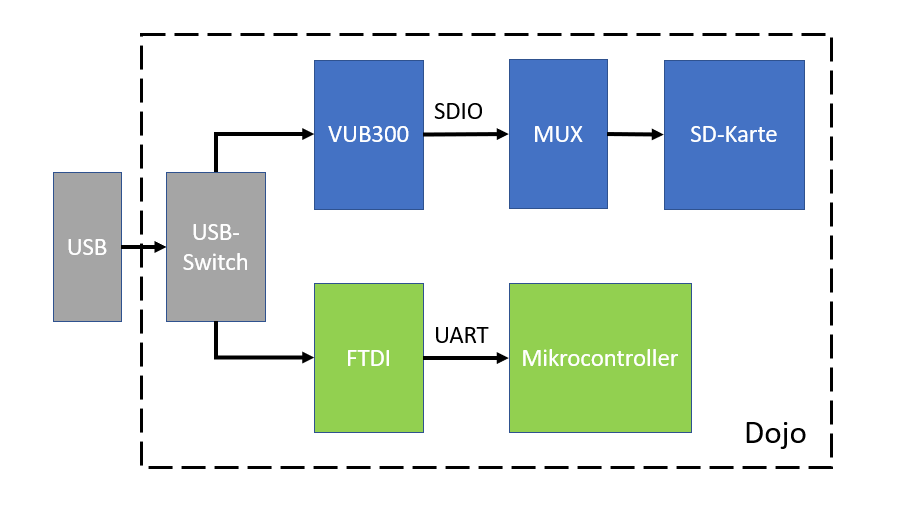
\includegraphics[width=\textwidth]{Bilder/Konzept_USB.PNG}
	\caption{Konzept USB}
	\label{Konzept_USB}
\end{figure}

Eine micro USB-Typ B Schnittstelle ist die gemeinsame Schnittstelle nach aussen. Dahinter schaltet ein USB-Switch, gesteuert durch den Mikrocontroller, einen der beiden Pfade durch. Es kann jeweils entweder der SDIO-Pfad oder UART-Pfad durchgeschaltet werden, nie beide Pfade gleichzeitig.\newline
Als USB-Switch wird der Baustein TS3USB30E von Texas Instruments verwendet. Dieser Chip wurde dafür entwickelt, um high-speed USB 2.0 Signale in portablen Geräten und Konsumelektronik zu schalten. Gesteuert wird der USB-Switch über zwei Pins. Über den Enable-Pin kann der Baustein in einen hochohmigen Zustand gebracht werden, um den Bus nicht zu belasten und den Stromverbrauch zu senken. Mit dem Select-Pin wird der durchzuschaltende Pfad ausgewählt.

Folgende Tabelle zeigt die Wahrheitstabelle für die entsprechenden Pfade:
\begin{figure}[h]
	\centering
	\begin{tabular}{|c|c|c|} 
		Select (Pin24) & $\overline{Enable}$ (Pin23) & Funktion \\ 
		\hline 
		X & HIGH & hochohmig \\ 
		\hline 
		LOW & LOW & Pfad = UART \\ 
		\hline 
		HIGH & LOW & Pfad = SDIO \\ 
	\end{tabular} 
	\caption{Wahrheitstabelle USB-Pfade}
	\label{truth_table_usb}
\end{figure}

\section{USB zu UART}

Der Baustein FT231X von FTDI stellt das Interface von USB zu UART bereit. Das ganze USB-Protokoll wird dabei auf dem Chip abgehandelt und es sind kaum zusätzliche Bauteile nötig (siehe Schema). Über zwei Pins (Rx und Tx) werden die Daten seriell übertragen.

Bei aktivem UART-Pfad wird der Dojo am Computer als serielle Schnittstelle erkannt. Über diese Schnittstelle kommuniziert nun die Software auf dem Computer mit dem Mikrocontroller im Gerät, um beispielsweise die \flq Likes\frq  auszulesen.


\section{USB zu SDIO}

Der VUB300 Chip vom Hersteller elan stellt das USB zu SDIO Interface bereit. Damit kann die SD-Karte im Dojo über den USB-Anschluss beschrieben und ausgelesen werden. Wird mit dem USB-Switch der SDIO-Pfad durchgeschaltet, erscheint die SD-Karte am Computer als Datenträger und kann gelesen sowie beschrieben werden. Zu beachten ist, dass zwischen dem VUB300 Chip und der SD-Karte noch ein weiterer Multiplexer (MUX) eingebaut ist. Mit diesem wird die SD-Karte zwischen dem VUB300 und dem Audio-Chip umgeschaltet. Genaueres dazu findet man in Abschnitt \textbf{\ref{Audioausgabe} \nameref{Audioausgabe}}.




\section{Validierung UART-Pfad}

Um die korrekte Funktion der seriellen Schnittstelle zwischen dem USB-Anschluss und dem Mikrocontroller zu überprüfen, wurde eine kleine Testsoftware auf den Mikrocontroller geladen. Sobald der Mikrocontroller am RX-Pin Zeichen empfängt, sendet	er diese über den TX-Pin wieder zurück. Mit dem Serial Monitor der Arduino IDE wurden die Zeichenketten erfolgreich gesendet und empfangen.

\section{Validierung SDIO-Pfad}

Mit einem weiteren Testprogramm wurde die Funktionsfähigkeit des SDIO-Pfades überprüft. Dafür wurde der USB-Switch und der MUX mit dem Mikrocontroller entsprechend angesteuert. Die SD-Karte wurde daraufhin von einem Computer mit Linux Betriebssystem als Datenträger erkannt und konnte ausgelesen und beschrieben werden. Leider stellte sich nach weiteren Tests heraus, dass auf einem Windows-Rechner keine SD-Karte erkannt wird. Die Gründe dafür sind nicht bekannt und das Problem konnte auch nicht behoben werden. Somit muss die Computer-Software auf einem Linux Betriebssystem gestartet werden.
\paragraph{Anmerkung}$ $\\
Durch die begrenzte Verfügbarkeit des VUB300 Chips, sowie der geringen Informationsdichte über den Baustein, ist dieser nicht für weitere Projekte oder Serienproduktionen zu empfehlen.